%\VignetteIndexEntry{Introduction to the geNet package}
%\VignetteEngine{R.rsp::tex}%\VignetteKeyword{R}
%\VignetteKeyword{package}%\VignetteKeyword{vignette}
%\VignetteKeyword{LaTeX}
\documentclass{article}
\usepackage{color, graphicx, setspace}
\usepackage{subfigure}
\usepackage{amsmath}
\usepackage{todonotes}
\usepackage{capt-of}
\usepackage{url}
\usepackage{float}
\usepackage[margin=0.5in]{geometry}
\usepackage[utf8]{inputenc}
\usepackage{hyperref}
\hypersetup{
    colorlinks=true, %set true if you want colored links
    linktoc=all,     %set to all if you want both sections and subsections linked
    linkcolor=blue,  %choose some color if you want links to stand out
}
\usepackage[nottoc,notlot,notlof]{tocbibind}
%\usepackage{caption}
%\usepackage{subcaption}
\usepackage{float}
\usepackage{listings}
\lstset{language=R,backgroundcolor=\color{gray}}
\usepackage{framed}

\begin{document}
\title{geNet: exploring large networks of genes}
\author{Sebastiano Montante}
\maketitle
\abstract{This vignette describes the main features of the geNet package. The geNet package is designed to measure the relationship between a pool of genes based on their occurrences across several strains. We also present a separate shiny app built on top of the geNet package visualization functions that allows an interactive exploration of large networks of genes}
\tableofcontents
\newpage






\section{Introduction}
The geNet tool is an R package that aims to generate an interactive network of genes in which each node is a gene and each edge measures the intensity of the relationship between two nodes.\\
The geNet package has two main components:
\begin{enumerate}
   	    	\item \textbf{The geNet algorithm}:
   	    	\begin{itemize}
   	    		\item Generating weightened connections of genes based on their occurences across several strains.
   	    		\item Clustering the nodes based on these weightened connections.
   	    	\end{itemize}
   	    	\item \textbf{A visualization framework} to easy navigate large networks of genes.
\end{enumerate}

The visualization framework includes a separate shiny app built on top of the geNet visualization framework functions that allows an interactive exploration of the network.


\begin{figure}[H]
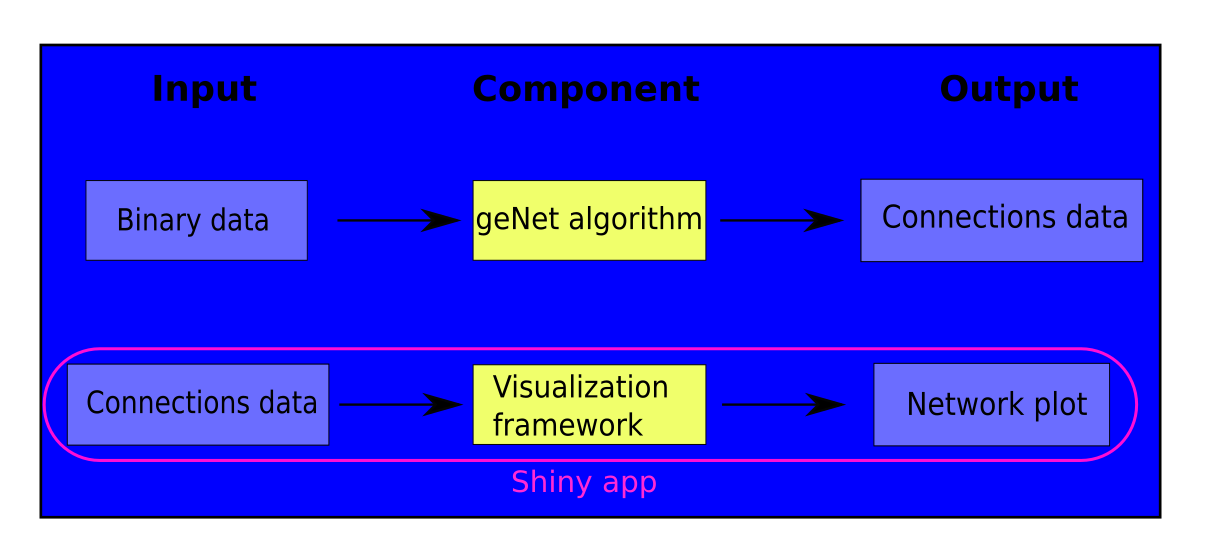
\includegraphics[width=15cm, height=8cm]{./Figures/geNet_package_summary.png}
\centering
\caption{General workflow of the two components of the geNet package}
\label{fig:genetworkflow}
\end{figure}

\newpage
\section{Installation}

geNet can be deployed using several methods: \\
\textbf{From source} \\
You can install geNet in your R environment from the source files (geNet.1.0.tar.gzip file) using the following R code:\\
\begin{framed}
\begin{lstlisting}
install.packages(``geNet.1.0.tar.gzip",repos=NULL,type=``source")
\end{lstlisting}
\end{framed}
However, the user needs to deal with packages installation and dependencies.\\
\textbf{From github}\\ 
The user can also install the package from Github using the command:\\
\begin{framed}
\begin{lstlisting}
devtools::install_github(``haneylab/geNet")
\end{lstlisting}
\end{framed}
\textbf{From a docker image}\\ 
A docker image of geNet is also available, one for the geNet package(genet.tar) and one for the shiny app (genetshiny.tar).
Once the docker file is downloaded, the user needs to load the image, for example in case you are loading the Shiny app image and the geNet image:
\begin{framed}
\begin{lstlisting}
sudo docker image load --input genetshiny.tar
sudo docker image load --input genet.tar
\end{lstlisting}
\end{framed}
Then the user must run a container (a instance of the image),for example:
\begin{framed}
\begin{lstlisting}
sudo docker run -e PASSWORD=1234 --rm -p 3838:3838 genetshiny:latest
sudo docker run -e PASSWORD=1234 --rm -p 8787:8787 genet:latest
# you can use -v tag to include a local folder in the docker container. For example:
sudo docker run -e PASSWORD=1234 --rm -p 8787:8787 -v /home:/home/rstudio/Home genet:latest
# It will the include the local home folder in your docker instance
\end{lstlisting}
\end{framed}
The geNet package container will run on localhost:8787 (accessible only from the local computer). You can change the port.\\
The Shiny app container will run using the Shiny Server. So it will run on IPaddress:3838, where IPaddress is the IP address of the server where the container is running. \\
You can see your Ip address from the terminal by executing:
\begin{framed}
\begin{lstlisting}
ip addr show
\end{lstlisting}
\end{framed}
If you are running the docker container inside a AWS instance, just use the IP address of you AWS instance.

\newpage
\section{geNet algorithm}
\subsection{Input}
The input to the geNet algorithm is a binary dataframe.
The rows names of this dataframe are the strains names.
The columns names of this dataframe are the nodes IDs (or genes ID) of the network. Indeed, each node of the network must be associated to a unique identifier that allows the algorithm to retrieve information about the nodes as described in "Visualization framework" section.\\
Before the execution of the actual geNet algorithm , a checking step is performed to assure that the input dataframe is formatted correctly.\\
The first checking step assures the absence of duplicated columns names. If duplicates are found, a message error is printed and the algorithm stops.
The second checking step assures that the values of the dataframe are binary. An integer 1 indicates the presence of the gene for a certain strain. An integer 0 indicates the absence of the gene. If the format does not match with this structure, a message error is printed and the algorithm stops.\\
As test data, the geNet package used a Pseudomonas strains presence/absence dataset.\\ 
In this dataset, the nodes IDs (i.e., the columns names) are the homologous gene families. There is a total of 24066 gene families, thus the node IDs ranges from 24066 to 1. The dataset reports the presence or absence of these gene families across 3093 strains. This dataset has been generated using the PyParanoid algorithm \cite{Melnyk2019}. \\
In order to get the annotation of these groups, the consesus sequences of each gene family have been mapped against a database of Pseudomonas references sequences, downloaded from the ``Pseudomonas Genome Database", containing only full complete sequences. ``Diamond" was used as mapping tool \cite{Buchfink2015}.


\subsection{Connections}
First, the geNet algorithm calculates the weighted connections between each node. In other words, the geNet algorithm measures the correlation for each combination of genes.
The correlation between each pair of genes is measured using the phi coefficient:
\begin{itemize}
	\item \textbf{The interpretation} of the phi coefficient is similar to the Pearson coefficient. Indeed, the Pearson coefficient applied to binary data with 2 categories gives the phi coefficient \cite{Jones2019}.
	\item The phi statistic is also a chi square based test whose \textbf{probability distribution is know}.  The phi statistic follows a chi-square probability distribution, thus the pvalue is calculated using the chi-square test (if the contingency table contains at least one value less than 5, the analogous fisher test is applied instead) \cite{Jones2019}.
\end{itemize}
Assuming the following 2x2 contingency table (table of frequencies for two categorical variables):\\
\begin{center}
\begin{tabular}{ c c c }
  & Var1=0 & Var1=1 \\ 
 Var2=0 & A & B \\  
 Var2=1 & C & D    
\end{tabular}
\end{center}
The formula to measure the phi coefficient is:\\
\begin{equation}
\phi=\frac{AD-BC}{(A+B)(C+D)(A+C)(B+D)}
\end{equation}
Considering $X^2=n\phi$:\\
\begin{equation}
\phi=\sqrt{\frac{X^2}{n}}
\end{equation}
Where $X^2$ is the chi-square statistic.\\

The chi-square distribution is the square of the z distribution (standard normal distribution) \cite{Huzak2011}. The Pearson correlation follows a t distribution.  With a large sample size, the t distribution and the z distribution (and thus the chi-square distribution) approximate very well the normal distribution \cite{Hazra2016}. Thus, the pvalue of the phi coefficient calculated using the Pearson correlaion significance test gives a good approximation of the real p-value when dealing with a large sample size.\\
geNet allows to calculate the p-value using both the chi square approach (chisq.test function or fisher.test function of the R stats package) or using the pearson correlation test (cor.test function of R stats package). The calculation based on the pearson correlation test is faster and is the default method.\\
In order to limit the false positives that can be generated by performing multiple comparisons like in this case, a Benjamini–Hochberg adjusment is applied to the p-values in next step.\\
By default the weights of the connections are the phi coefficients, but the user can also choose to use as weight the negative log-pvalues. The coefficient measures the intensity of the correlation, while the p-value measures the significance of the correlation \\
Finally, the geNet algorithm filters the p-values and the coefficients to exclude the not relevant connections.\\
By default, the filtering of the pvalues is conservative and considers only the p-values less than 0.01. Thus, the algorithm considers only the highest significant connections. The user can select an higher threshold of significance. 
The threshold for the filtering of the coefficients is automatically estimated from the data and is equal to
$u + 3*sd$ where $u$ is the mean of the coefficients and $sd$ is the standard deviation. All coefficients inferior to this threshold are filtered out.\\
Note that this filtering applies only to the positive edges,the negative edges are not involved in the clustering algorithm and they don't influence the topology of the network. By default, the negative edges with a p-value above 0.1 are filtered out. The negative edges with a coefficient absolute value near 0($<0.02$) are filterted out.
The geNet algorithm is implemented using the ff and ffbase packages to reduce the burden of large data objects on the RAM memory. Parallel computing is also implemented to speed up the algorithm execution.\\


% Reference: http://web.pdx.edu/~newsomj/uvclass/ho_correlation%20t%20phi.pdf

\newpage
\subsection{Clustering}
The final step of the geNet algorithm uses a clustering algorithm to group the nodes in communities (clusters or modules) based on the weights of the connections calculated in the first step.\\
A network community is defined as a group of nodes that interact more often between themselves than with nodes from other groups \cite{Linhares2020}.\\
Choosing an "absolute" optimal clustering algorithm is not feasible and the user may want to test different clustering algorithms (the visualization framework allows the user to test 4 different clustering algorithms).
The most common meausures to evalute a clustering algorithm are: Precision, Recall, F-measure and Modularity \cite{Linhares2020}.
However, the first three requires the presence of ground-truth labels. In other words, the user already knows the correct communities.  Modularity does not require a pre-defined information regarding the communities \cite{Linhares2020}. geNet is designed to be an exploratory tool and so the modularity could be a good measure to evaluate the clustering of the nodes. The modularity is defined as \cite{Linhares2020}:\\
\begin{equation}
M=\frac{1}{2W} \sum\nolimits_{ij}[w_{ij} - \frac{k_{j}k_{i}}{2W}]\delta(c_i,c_j)
\end{equation}
Where:\\
$w_{ij}$ is the edge weight between nodes $i$ and $j$\\
$k_i$ is the sum of the weights of links that connect to node $i$ \\
$W$ is the sum of the weights of all links in the network\\
$c_i$ is the community of node $i$\\
$\delta(c_i,c_j)$ is the delta function: if $c_i==c_j$ $1$ else $0$\\
Networks with high modularity have dense connections between the nodes within the same communities (these nodes have more interactions) but sparse connections between nodes in different communities (these nodes have less interactions).\\
The Louvain algorithm is an unsupervised learning algorithm (i.e., a community detection algorithm) designed to maximize the modularity (i.e., it optimizes the modularity objective function to find a global maximum).\\
The Louvain training is divided in two steps plus an initialization step.\\
During the initialization step the Louvain algorithm assigns each node to a community.\\
In step 1,  each node $i$ is assigned to the community of each of its neightbors, for each movement the difference in modularity is calculated.  In the end, the node $i$ is assigned to the community with the highest modularity gain. If there is no positive increase, the node $i$ remains in its original. These steps are repeated for each node and until the modularity does not increase anymore.
Then  step 2 starts. The new communities becomes the nodes of a new network.  The weight of a link between two nodes is the sum of the weights of all the links between the nodes in the corresponding communities.
Step 1 and step 2 are repeated until a maximum modularity value is reached. 

The Louvain algorithm has some drawbacks.
There is a resolution limit. The smaller communities may be hidden by the bigger communities. In addition, the global maximum found by the Louvain algorithm may not be the most relevant suddivision in terms of scientific results. Indeed, the smaller communities may be more important than the bigger communities \cite{Linhares2020}.\\

The Infomap algorithm is another widely used community detection algorithm. The Infomap does not use the modularity but tries to solve the clustering problem using a random walker \cite{Linhares2020}.\\
In particulars it measures the time the random walker spends within a group of nodes. The network structure is then represented by a Huffman code (i.e. each node and communities is assigned to a binary sequence) and the optimal community structure is given by detecting the communities in which the random walker gets trapped more often \cite{Linhares2020}.\\
The algorithm minimize an objective function called "map equation"(in other words it minimizes the description lenght of a random walker) \cite{Linhares2020}:\\
\begin{equation}
L(M)=q_{between}H(Q) + \sum\limits_{i=1}^m p_{within}^{i}H(P^{i})
\end{equation}
Where:
$q_{between}H(Q)$ indicates the average number of bits necessary to describe movement between communities\\
$\sum\limits_{i=1}^m p_{within}^{i}H(P^{i})$ indicates the average number of bits necessary to describe movement within communities.\\
$q_{between}=\sum\limits_{i=1}^m q_{i,between}$ Per-step probability that the random walker switches modules.\\ 
$q_{i,between}$ is the per-step probability that the walker leaves module $i$.\\
$H(Q)$ is the entropy of movement between modules.\\
$H(P^{i})$ is the entropy of movement within modules.\\
$p_{within}^{i}$ weights $H(P^{i})$ based on the frequency of the random walker visiting node $i$.\\
The optimization process is similar to the Louvain algorithm.\\
Initialiation: randomly assignation of each node $i$ to a different community\\
Step 1: Moving nodes to neighboring communities for greatest decrease in L\\
Step 2: aggregating communities in nodes\\
Repeating step 1 and step 2 until $L$ is minimized.\\
In summary, there is no "absolute" optimal solution and the visualization framework of geNet provides a user-friendly way to test different clustering methods. By defaul the geNet algorithm uses the Infomap algorithm to avoid hiding the smaller communities (the modularity value returned is not the global maximum).\\
The output of the geNet algorithm is a list of ffdf objects (ffdf is a dataframe-like structure generated using the ff package). This object contains the information about the connections between the nodes of the network and the association of the nodes with the clusters. It is possible to export this object using the export\_ geNet\_ output() function.\\
Here's a minimum example of a correct execution of the geNet algorithm:
\begin{framed}
\begin{lstlisting}
library(geNet) # Importing the geNet package
# Importing the binary dataframe that reports the occurences of the genes across the strains.
path_binary_df<-system.file("extdata", "bn_df_test.csv", package = "geNet")
bn_df<- read.csv(file=path_binary_df,row.names=1) # first column contains the row names (strains names)
data_connections<-geNet(input_binary_df=bn_df,cores=1) # we execute the geNet algorithm
# Depending on the number of genes and cores, it may take from few minutes to several hours)
# In case we want to export the results outside the R enviroment, we execute:
export_geNet_output(geNet_output=data_connections,out_directory=path)
# where path is the full path of the directory where the results must be exported
\end{lstlisting}
\end{framed}

All geNet functions and relative arguments are reported in geNet\_functions.pdf.\\


\newpage
\section{Visualization framework}
The visualization framework is enterely based on the famous visNetwork R package that allows an high interactive visualization of networks.\\
However, with a large number of nodes, displaying directly the full network of nodes with all edges for each node is both unfeasible and unuseful. Large networks tends to form heavily condensed clusters where all nodes are connected to each other. The visualization of nodes and edges may be confusing and the contribution of the single edge is not relevant anyway. The researchers can get more information  by analyzing the relationships between the clusters.\\
Thus, geNet provides a series of visualization functions that allows an immediate expansion and contraction of the network clusters based on the researcher input. The visualization functions allows also to get several information about the clusters and the connections between the nodes of different clusters.\\
In the shiny enviroment, the application of the visualization functions occurs interactively providing an user-friendly tools to explore the relationship between the nodes of the network.
Here's a minimum example of a correct execution of the visualization functions:
\begin{framed}
\begin{lstlisting}
library(geNet) # Importing the geNet package
# plot the network of clusters
plot_visnetwork(data=data_connections, contract_net=T)
# Now, maybe we want to see the network of genes of one group.
# we get the vector containing all groups names
all_groups<-unique(data_connections$nodes$group[])
# we get the data for the first group
data_connections_group_1<-visualize_network(data=data_connections,
select_group=all_groups[1])
# we plot this group visualizing the positive edges...
plot_visnetwork(data=data_connections_group_1, contract_net=F,show_negative=F)
#... or the negative edges
plot_visnetwork(data=data_connections_group_1, contract_net=F,show_negative=T)
\end{lstlisting}
\end{framed}
There are many several options to navigate the connections, see geNet\_functions.pdf for a detailed explanation.\\
For example: by default the clusters are named based on a random color assigned during the geNet algorithm execution. If you want to name the clusters based on the number of nodes you can execute:
\begin{framed}
\begin{lstlisting}
library(geNet) # Importing the geNet package
df_new_groups_names<-get_group_names_based_on_n_nodes(data=data_connections)
data_connections_renamed<-mod_group_names(data=data_connections,df_new_groups_names=df_new_groups_names)
plot_visnetwork(data=data_connections_renamed, contract_net=T)
\end{lstlisting}
\end{framed}
The shiny app combines all the visualization functions in an interactive way to make the experience even more user friendly.
Here's a scheme of the shiny app algorithm:

\begin{figure}[H]
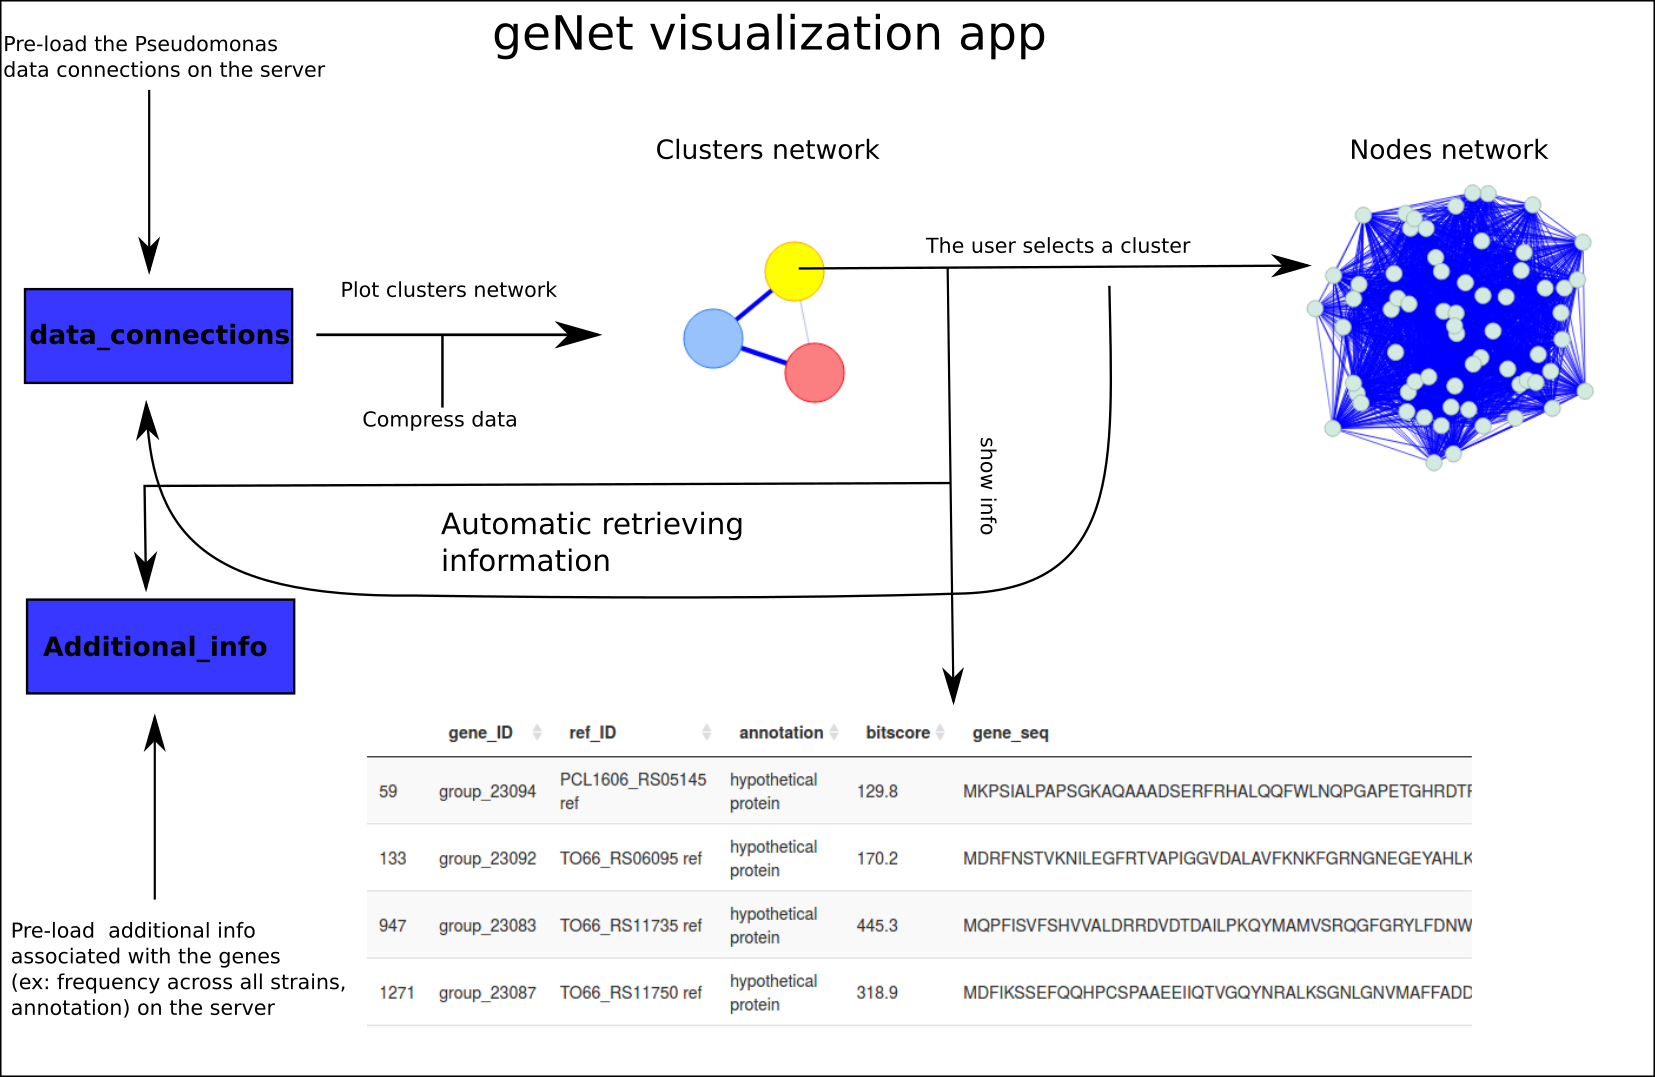
\includegraphics[width=18cm, height=10cm]{./Figures/visualization_framework_scheme.png}
\centering
\caption{Shiny app of the geNet visualization framework}
\label{fig:genetvisualization}
\end{figure}

The data containing the connections and the clustering information (generated using the geNet algorithm with default options) is pre-loaded by the Shiny app. A dataframe containing additional information about the nodes (e.g., annotation,frequency across the strains etc...) is also pre-loaded.\\
Then, the clusters network is automatically plotted immediately after the end of the pre-loading step (Note: only connected groups are shown).
The plotting of the clusters network generates an intermediate data object. This object is a compressed version of the original data and contains only the information related to the connections between the clusters and which nodes belong to each cluster. It does not contain any information regarding how the nodes are connected within the clusters. This compression allows the plotting of the clusters network in a relative short time (around 4 minutes).\\
When the user sends to the server the request to visualize  
one or more clusters, the server automatically looks for these clusters in the original data containing the nodes connections information and plot them.
The server can plot only a maximum of 1000 nodes, if the user tries to plot a network with a number of nodes greater than 1000 an error message is returned.
The shiny app allows a fast retrieve of several information about the clusters avoiding the need to plot the network. By clicking on one cluster, the content of that cluster is shown (i.e., the list of nodes inside the cluster). By double clicking a cluster the connections in common between the selected cluster and the other clusters are shown. The shiny app includes several other visualization options, the help section of the app describes these options.

\bibliography{Bibliography_references}
\bibliographystyle{ieeetr}
\end{document}